 %%%%%%%%%%%%%%%%%%%%%%%%%%%%%%%%%%%%%%%%%
% Beamer Presentation
% LaTeX Template
% Version 1.0 (10/11/12)
%
% This template has been downloaded from:
% http://www.LaTeXTemplates.com
%
% License:
% CC BY-NC-SA 3.0 (http://creativecommons.org/licenses/by-nc-sa/3.0/)
%
%%%%%%%%%%%%%%%%%%%%%%%%%%%%%%%%%%%%%%%%%

%----------------------------------------------------------------------------------------
%	PACKAGES AND THEMES
%----------------------------------------------------------------------------------------

\documentclass{beamer}

\mode<presentation> {

% The Beamer class comes with a number of default slide themes
% which change the colors and layouts of slides. Below this is a list
% of all the themes, uncomment each in turn to see what they look like.

%\usetheme{default}
%\usetheme{AnnArbor}
%\usetheme{Antibes}
%\usetheme{Bergen}
%\usetheme{Berkeley}
%\usetheme{Berlin}
%\usetheme{Boadilla}
\usetheme{CambridgeUS}
%\usetheme{Copenhagen}
%\usetheme{Darmstadt}
%\usetheme{Dresden}
%\usetheme{Frankfurt}
%\usetheme{Goettingen}
%\usetheme{Hannover}
%\usetheme{Ilmenau}
%\usetheme{JuanLesPins}
%\usetheme{Luebeck}
%\usetheme{Madrid}
%\usetheme{Malmoe}
%\usetheme{Marburg}
%\usetheme{Montpellier}
%\usetheme{PaloAlto}
%\usetheme{Pittsburgh}
%\usetheme{Rochester}
%\usetheme{Singapore}
%\usetheme{Szeged}
%\usetheme{Warsaw}

% As well as themes, the Beamer class has a number of color themes
% for any slide theme. Uncomment each of these in turn to see how it
% changes the colors of your current slide theme.

%\usecolortheme{albatross}
%\usecolortheme{beaver}
%\usecolortheme{beetle}
%\usecolortheme{crane}
%\usecolortheme{dolphin}
%\usecolortheme{dove}
%\usecolortheme{fly}
%\usecolortheme{lily}
%\usecolortheme{orchid}
%\usecolortheme{rose}
%\usecolortheme{seagull}
%\usecolortheme{seahorse}
%\usecolortheme{whale}
%\usecolortheme{wolverine}

%\setbeamertemplate{footline} % To remove the footer line in all slides uncomment this line
%\setbeamertemplate{footline}[page number] % To replace the footer line in all slides with a simple slide count uncomment this line

%\setbeamertemplate{navigation symbols}{} % To remove the navigation symbols from the bottom of all slides uncomment this line
}

\usepackage{graphicx} % Allows including images
\usepackage{booktabs} % Allows the use of \toprule, \midrule and \bottomrule in tables

%----------------------------------------------------------------------------------------
%	TITLE PAGE
%----------------------------------------------------------------------------------------

\title[Diabetic Retinopathy]{Vessel segmentation in Retinal Images } % The short title appears at the bottom of every slide, the full title is only on the title page

\author{Kushal Khandelwal} % Your name
\institute[HCI/IWR] % Your institution as it will appear on the bottom of every slide, may be shorthand to save space
{
University of Heidelberg \\ % Your institution for the title page
\medskip
\textit{kushal.khandelwal@iwr.uni-heidelberg.de} % Your email address
}
\date{\today} % Date, can be changed to a custom date

\begin{document}

\begin{frame}
\titlepage % Print the title page as the first slide
\end{frame}

% \begin{frame}
% \frametitle{Overview} % Table of contents slide, comment this block out to remove it
% \tableofcontents % Throughout your presentation, if you choose to use \section{} and \subsection{} commands, these will automatically be printed on this slide as an overview of your presentation
% \end{frame}

%----------------------------------------------------------------------------------------
%	PRESENTATION SLIDES
%----------------------------------------------------------------------------------------

%------------------------------------------------
\section{Problem Statement} % Sections can be created in order to organize your presentation into discrete blocks, all sections and subsections are automatically printed in the table of contents as an overview of the talk
%------------------------------------------------

\subsection{Description} % A subsection can be created just before a set of slides with a common theme to further break down your presentation into chunks

\begin{frame}
\frametitle{Retinal Vessel Segmentation}

\begin{columns}[c] % The "c" option specifies centered vertical alignment while the "t" option is used for top vertical alignment

\column{.45\textwidth} % Left column and width

Retinal vessel segmentation in digital fundus images for development of automatic screening systems for diabetic retinopathy.

\column{.5\textwidth} % Right column and width
\begin{figure}
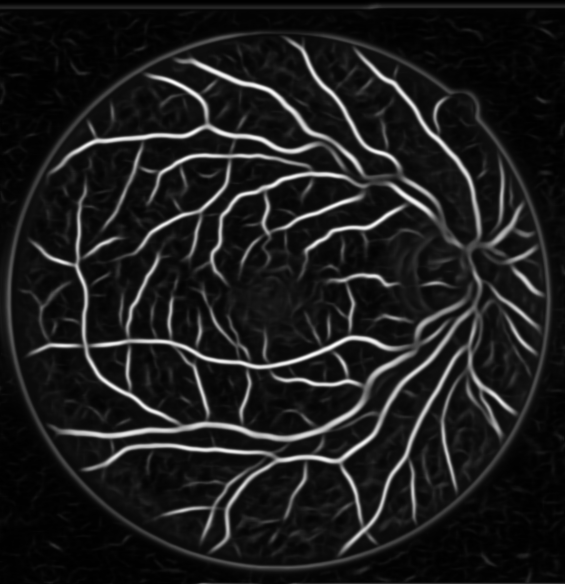
\includegraphics[width=0.6\linewidth]{Images/slide1.png}
\end{figure}

\end{columns}



\end{frame}

%------------------------------------------------

% \begin{frame}
% \frametitle{Why is it important ?}

% Mitosis Detection in images of H and E stained slides of breast cancer.

% \end{frame}

\subsection{Task}
\begin{frame}
\begin{figure}
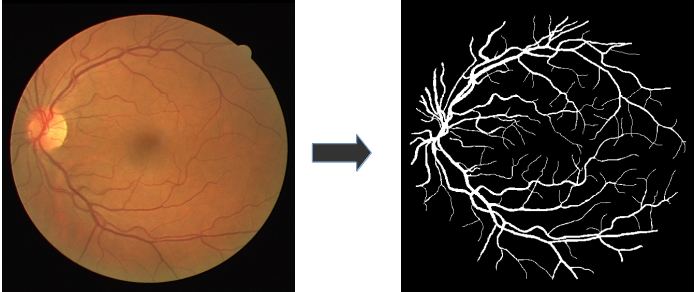
\includegraphics[width=1.0\linewidth]{Images/Graphic1.png}
\end{figure}
\end{frame}
%------------------------------------------------
\subsection{Importance}
\begin{frame}
\frametitle{Why is it important ?}
\begin{itemize}
\item To calculate the morphological attributes of the retinal vessels(length, width)
\item Vessel diameter measurement helpful for diagnosis of hypertension
\item Retinal vascular tree is unique,and can be used for biometric purposes

\end{itemize}
\end{frame}

%------------------------------------------------

\subsection{Challenges}
\begin{frame}
\frametitle{Limitations of Current Methods}
\begin{itemize}
\item Merging of close vessels
\item False vessel detection
\item Segmentation at Bifurcation and Crossover regions
\item Poor detection of thin vessels

\end{itemize}
\end{frame}

%------------------------------------------------
\subsection{Task}
\begin{frame}
\begin{figure}
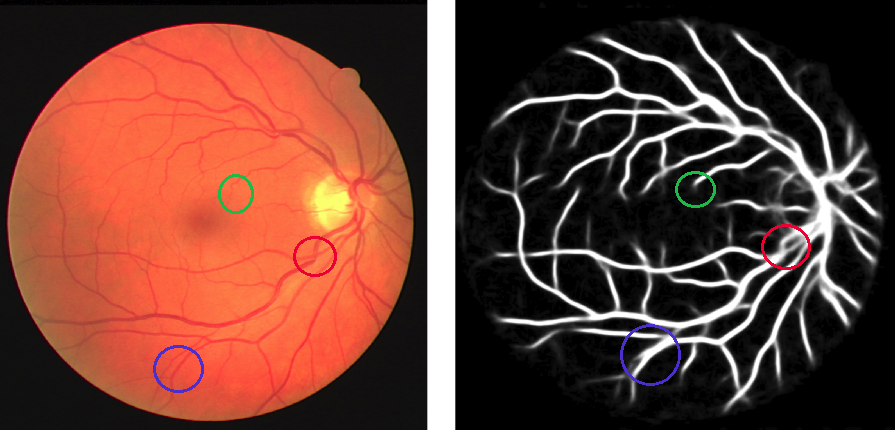
\includegraphics[width=1.0\linewidth]{Images/problem1.png}% Insert Image with cropping
\end{figure}
\end{frame}
%------------------------------------------------
%----------------------------------------------%
%%%%%%%%%%%%%%%%%%%%%%%%%%%%%%%%%%%%%%%%%%%%%%%%%%
\section{Related Work}
%%%%%%%%%%%%%%%%%%%%%%%%%%%%%%%%%%%%%%%%%%%%%%%%%%
\subsection{Related Work}


\begin{frame}
\frametitle{Related Work}
There has been a lot of work on retinal image segmentation. Some of them are :
\begin{itemize}
\item Tracking techniques to trace vessels starting from some seed points.
\item Staal et al, presented a ridge based vessel segmentation methods.
\item Ricci and Perfetti proposed a methodology using line operators as feature vectors and SVM for pixel classification.
\item Osareh and Shadgar used multiscale Gabor filters for vessel candidate identification.
\item Most of the methods utilize some sort of pixel level features and learn a classifier for classifying pixels as vessel or background.
\end{itemize}
\end{frame}
%---------------------------
\subsection{Related Work}

\begin{frame}
\frametitle{Related Work}
Some of the recent works we compare our model to are :
\begin{itemize}

\item Structured Forests for Fast Edge Detection (SE) [Dollar et al]
\item Accurate and Efficient Linear Structure Segmentation by leveraging Ad Hoc Features with learned Filters (CS) [Rigamonti et al]
\item Filter Learning for Linear Structure Segmentation (DL) [R.Rigamonti]
\item Neural Network Nearest Neighbor Fields for Image Transforms (N4) [Ganin et al]
\end{itemize}

\end{frame}

%------------------------------------------------------%


%------------------------------------------------------%
\subsection{SE}

\begin{frame}
\frametitle{Structured Forests}
\begin{columns}[c] % The "c" option specifies centered vertical alignment while the "t" option is used for top vertical alignment

\column{.55\textwidth} % Left column and width
\begin{itemize}
\item Takes advantages of the presence of well known forms like  T-junctions,Y-Junctions, Straight lines exhibited by edges in local patches. They train random forests in a structured learning setting.
\item DRIVE Dataset AUC  = 0.90
\end{itemize}

\column{.4\textwidth} % Right column and width
\begin{figure}
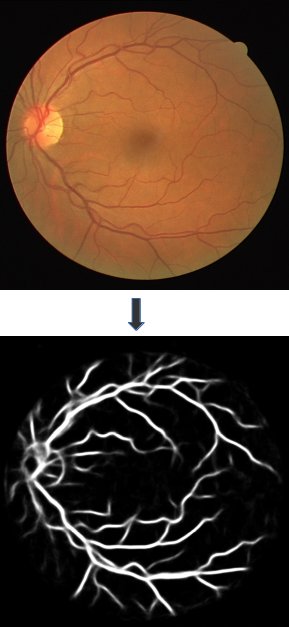
\includegraphics[width=0.6\linewidth]{Images/SE.png}
\end{figure}

\end{columns}

\end{frame}


%------------------------------------------------------%

\subsection{CS}

\begin{frame}
\frametitle{Ad Hoc Features and Learned Filters}
\begin{columns}[c] % The "c" option specifies centered vertical alignment while the "t" option is used for top vertical alignment

\column{.4\textwidth} % Right column and width
\begin{figure}
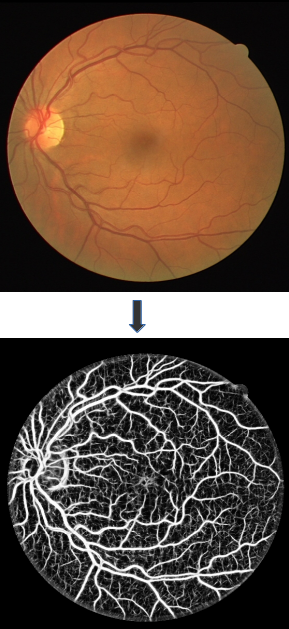
\includegraphics[width=0.6\linewidth]{Images/CS.png}
\end{figure}

\column{.55\textwidth} % Left column and width
\begin{itemize}
\item Linear filters are learned by modeling the distribution of image representatives.
\item Features maps are computed using the learned filters and other hand crafted features  are computed.
\item A random forest classifier is trained to classify each image location as lying on a linear structure or background.
\item DRIVE Dataset AUC  = 0.95
\end{itemize}



\end{columns}

\end{frame}




%------------------------------------------------------%

%------------------------------------------------------%

\subsection{DL}

\begin{frame}
\frametitle{Filter Learning for Linear Structure Segmentation}
\begin{columns}[c] % The "c" option specifies centered vertical alignment while the "t" option is used for top vertical alignment



\column{.55\textwidth} % Left column and width
\begin{itemize}
\item Linear filters are learned in form of a dictionary.
\item Features maps are computed using the learned filters
\item A random forest classifier is trained to classify each image location as lying on a linear structure or background.
\item DRIVE Dataset AUC = 0.95
\end{itemize}

\column{.4\textwidth} % Right column and width
\begin{figure}
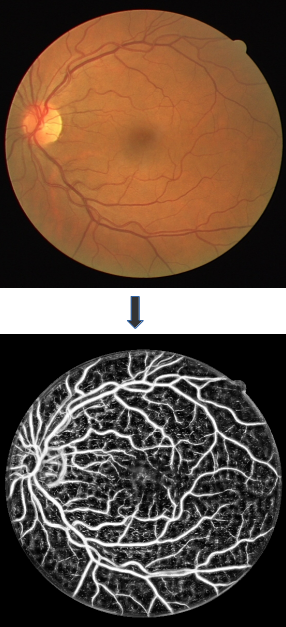
\includegraphics[width=0.6\linewidth]{Images/DL.png}
\end{figure}

\end{columns}

\end{frame}




%------------------------------------------------------%
%------------------------------------------------------%

\subsection{N4}

\begin{frame}
\frametitle{Neural Network Nearest Neighbor Fields for Image Transforms}
\begin{columns}[c] % The "c" option specifies centered vertical alignment while the "t" option is used for top vertical alignment

\column{.4\textwidth} % Right column and width
\begin{figure}
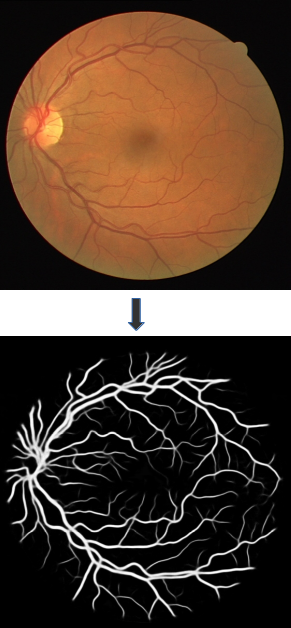
\includegraphics[width=0.6\linewidth]{Images/N4.png}
\end{figure}

\column{.55\textwidth} % Left column and width
\begin{itemize}
\item CNN is trained to learn an intermediate mapping for the patches. Each patch is mapped to an intermediate annotation map.
\item For a given set of intermediate mapping of training patches, a dictionary is learned mapping to the GT patches.
\item New input patches are assigned annotation from the dictionary patch with the closest CNN output.
\item DRIVE Dataset AUC = 0.97 
\end{itemize}



\end{columns}

\end{frame}

\subsection{Results}
\begin{frame}
\frametitle{Results}

\begin{figure}
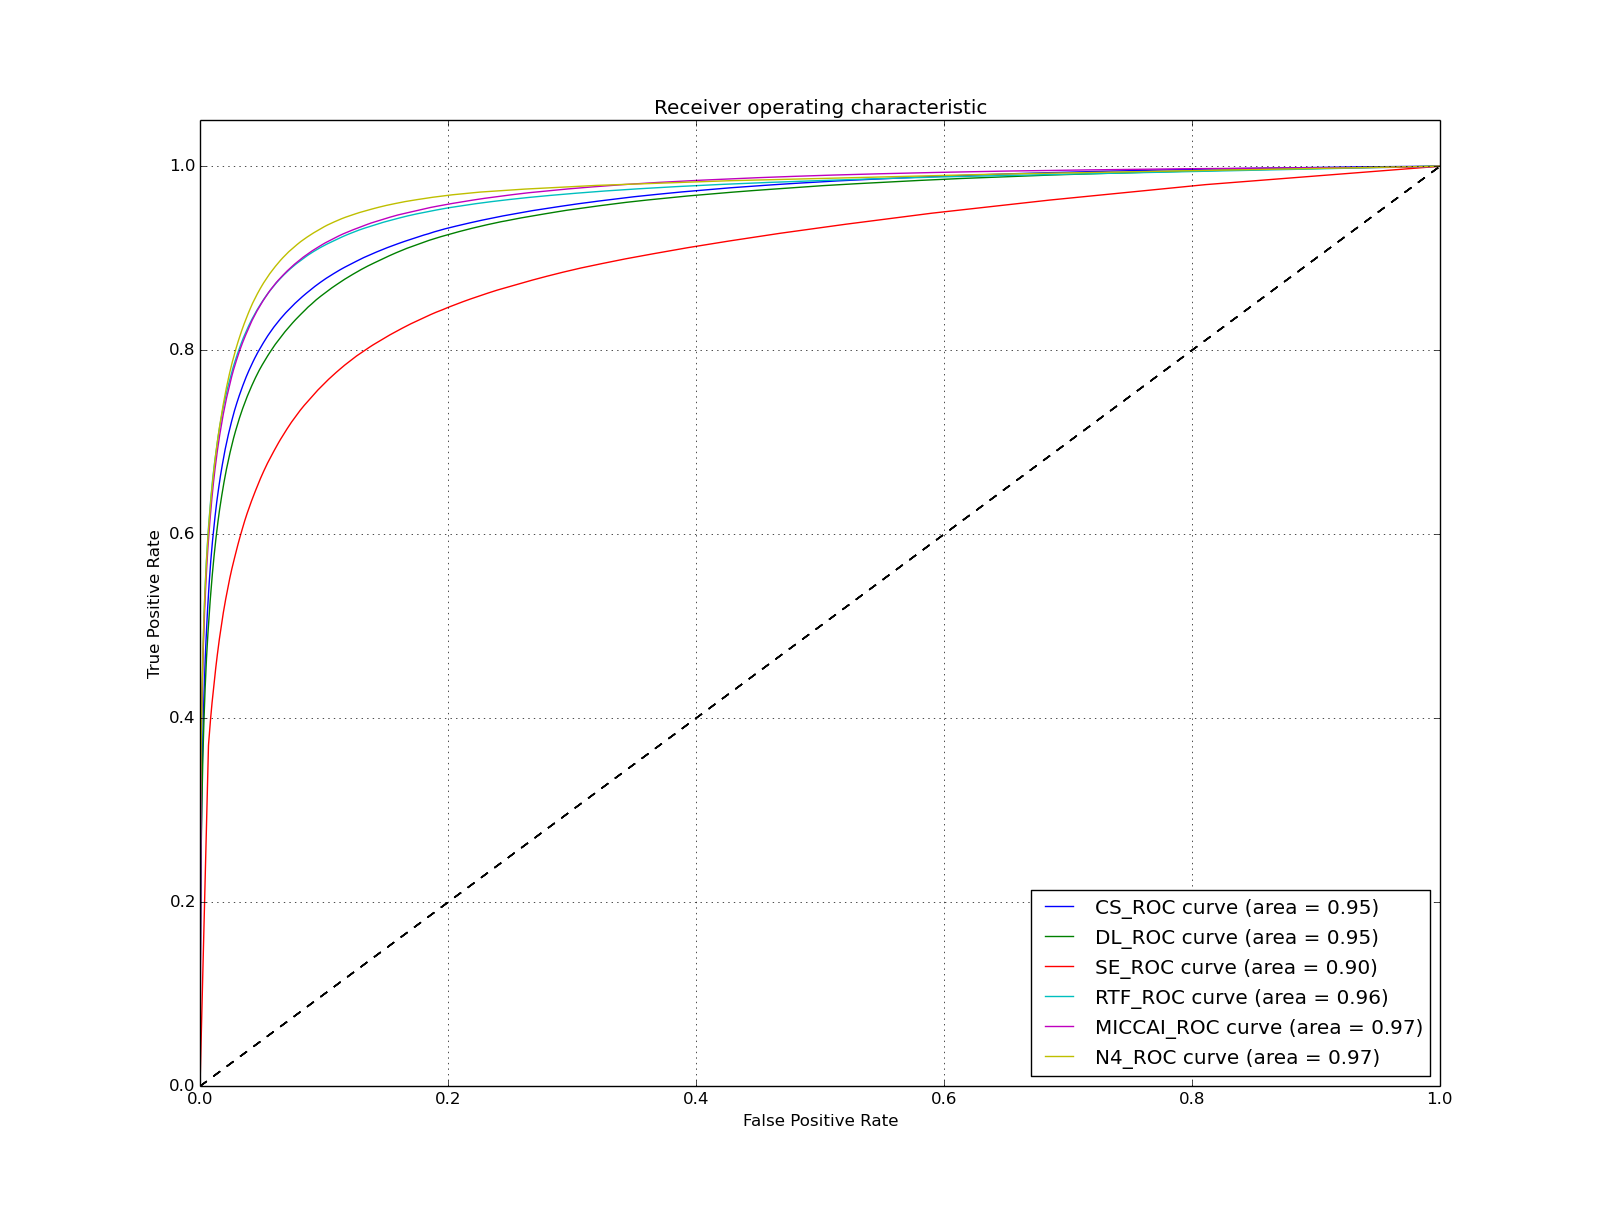
\includegraphics[width=0.8\linewidth]{Images/othermethods.png}
\end{figure}
\end{frame}


%------------------------------------------------------%
\section{Proposed Method}
%------------------------------------------------------%
%------------------------------------------------------%
%------------------------------------------------------%
\subsection{Method}
\begin{frame}
\frametitle{Proposed Method}
In the proposed method, pixel classification is done by learning clusters from raw pixels and associating them with ground truth patches.

We are given a set of Images I, ground truth G and mask M
\begin{figure}
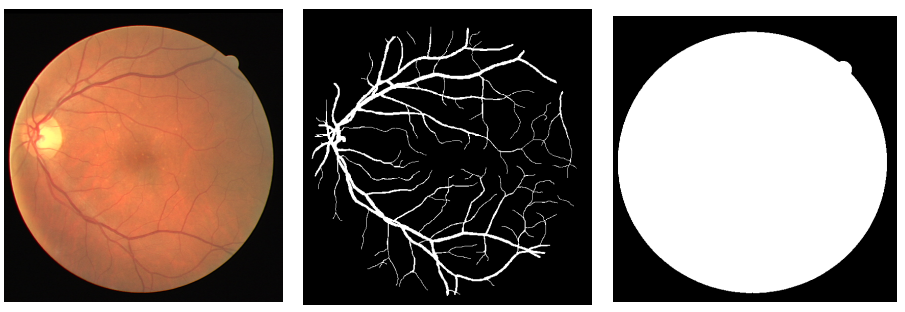
\includegraphics[width=1.0\linewidth]{Images/Method1.png}
\end{figure}
\end{frame}

%------------------------------------------------
\subsection{Method}
\begin{frame}
\frametitle{Proposed Method - Patching}
\begin{itemize}
\item For each channel of the image I and GT image G, we compute patches at each image pixel. Vectorize all the patches.
\begin{figure}
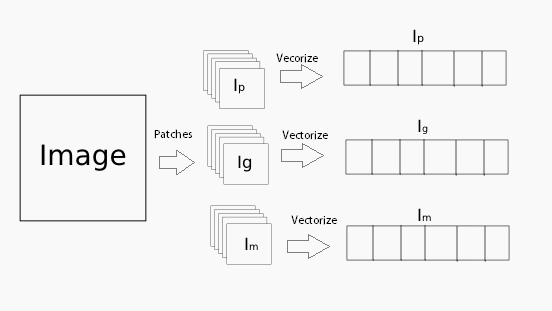
\includegraphics[width=0.8\linewidth]{Images/Method2.png}

\end{figure}


\end{itemize}

\end{frame}
%------------------------------------------------
\subsection{Method}
\begin{frame}
\frametitle{Proposed Method - Patch Selection}
\begin{itemize}
\item Select a subset of patches with more than 50\% inside the mask region. 
\item From this set of useful patches we select X\% of patches for clustering.
 corresponding cluster.
\end{itemize}
\begin{figure}
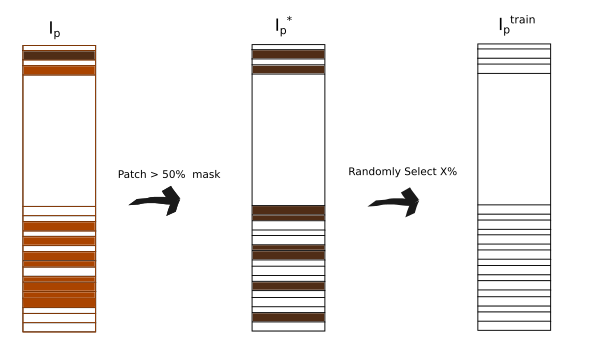
\includegraphics[width=0.8\linewidth]{Images/method3.png}

\end{figure}


\end{frame}

%------------------------------------------------

\subsection{Method}
\begin{frame}
\frametitle{Proposed Method - Clustering}
\begin{itemize}
\item The selected patches for each channel are then clustered into K clusters using Kmeans Clustering.
\item We then create an inverted list mapping each patch to a cluster.
\item For each patch associated to a cluster, its corresponding GT patch is assigned to the cluster.
\item All the ground truth patches for a given cluster are averaged to get the Ground Truth image for the corresponding cluster.
\end{itemize}

\end{frame}
%------
\subsection{Method}
\begin{frame}
\frametitle{Clusters}
\begin{figure}
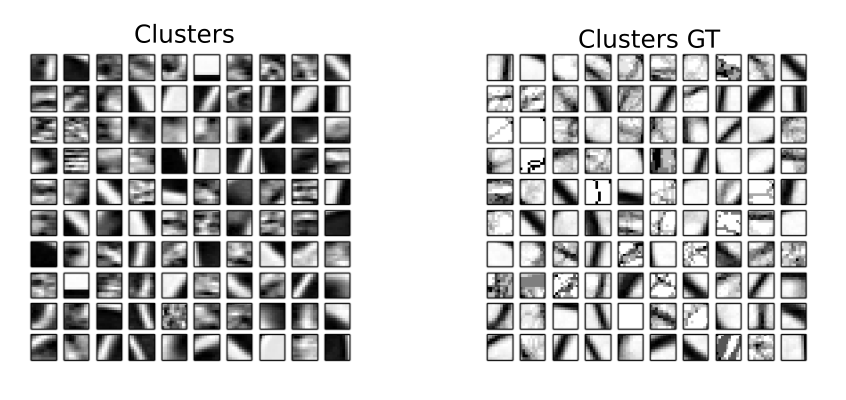
\includegraphics[width=1.0\linewidth]{Images/methodclus.png}

\end{figure}

\end{frame}
%-------------------------------------
\subsection{Method}
\begin{frame}
\frametitle{Prediction on a New Image}
\begin{itemize}
\item Given a new images, patches for each channel are created.
\item For each patch the cluster is predicted based on minimum distance from the clusters.
\item Each patch is the replaced by the GT image of the cluster.
\item All the patches are aggregated to obtain the segmented image.
\end{itemize}

\end{frame}
\subsection{Method}
\begin{frame}
\frametitle{Predictions}
\begin{figure}
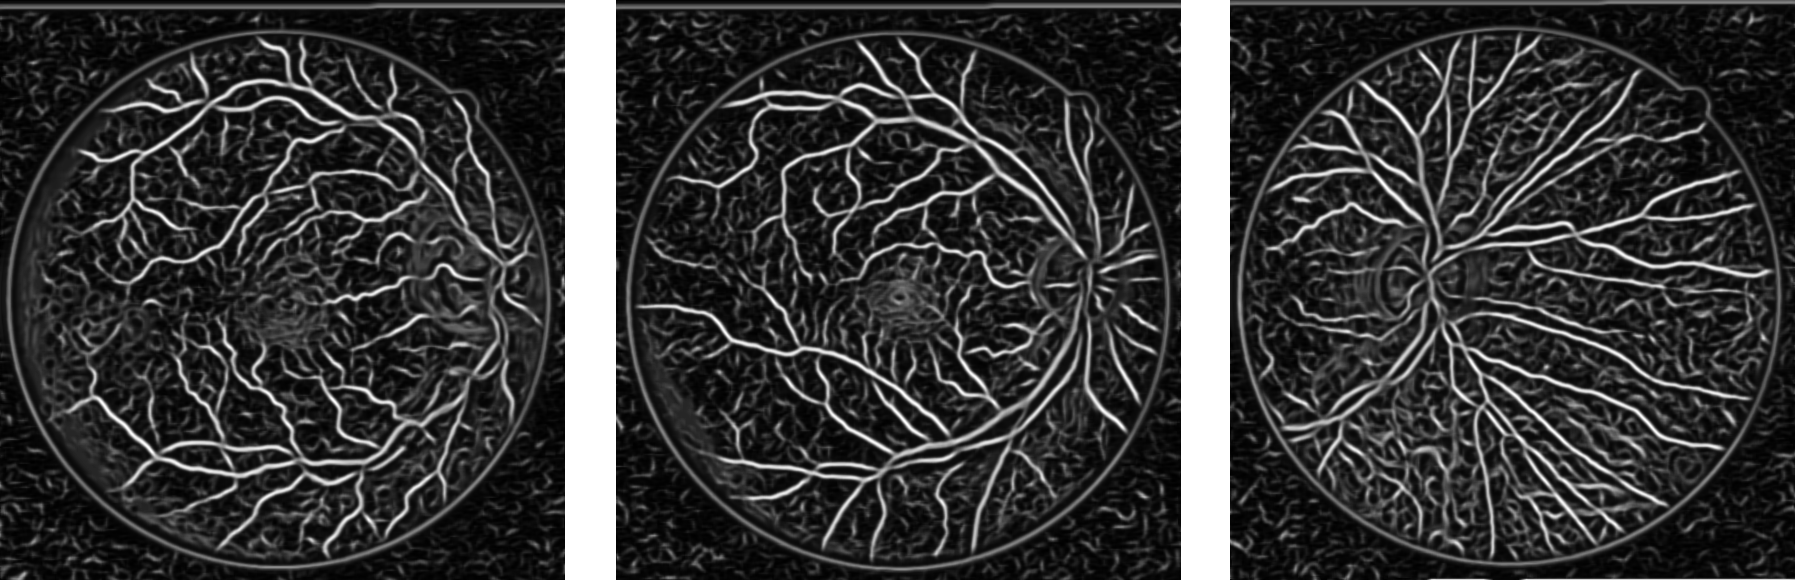
\includegraphics[width=1.0\linewidth]{Images/new.png}

\end{figure}

\end{frame}
%------------------------------------------------
\section{Dataset}
%------------------------------------------------

\begin{frame}
\frametitle{Dataset}
The experiments were performed on the following datasets:
\begin{table}
\begin{tabular}{l l l l}
\toprule
\textbf{Dataset} &  \textbf{Total Images} & \textbf{Training Images} & \textbf{Test Images}\\
\midrule
DRIVE & 40 & 20 & 20  \\
STARE & 20 & 10 & 10 \\


\bottomrule
\end{tabular}
\end{table}


\end{frame}

%------------------------------------------------

%------------------------------------------------
\section{Experiments}
%------------------------------------------------
\subsection{Expt-1}
\begin{frame}
\frametitle{Comparison with other methods}
We perform clustering with K=1000 and patchsize =(10,10). 
\begin{figure}
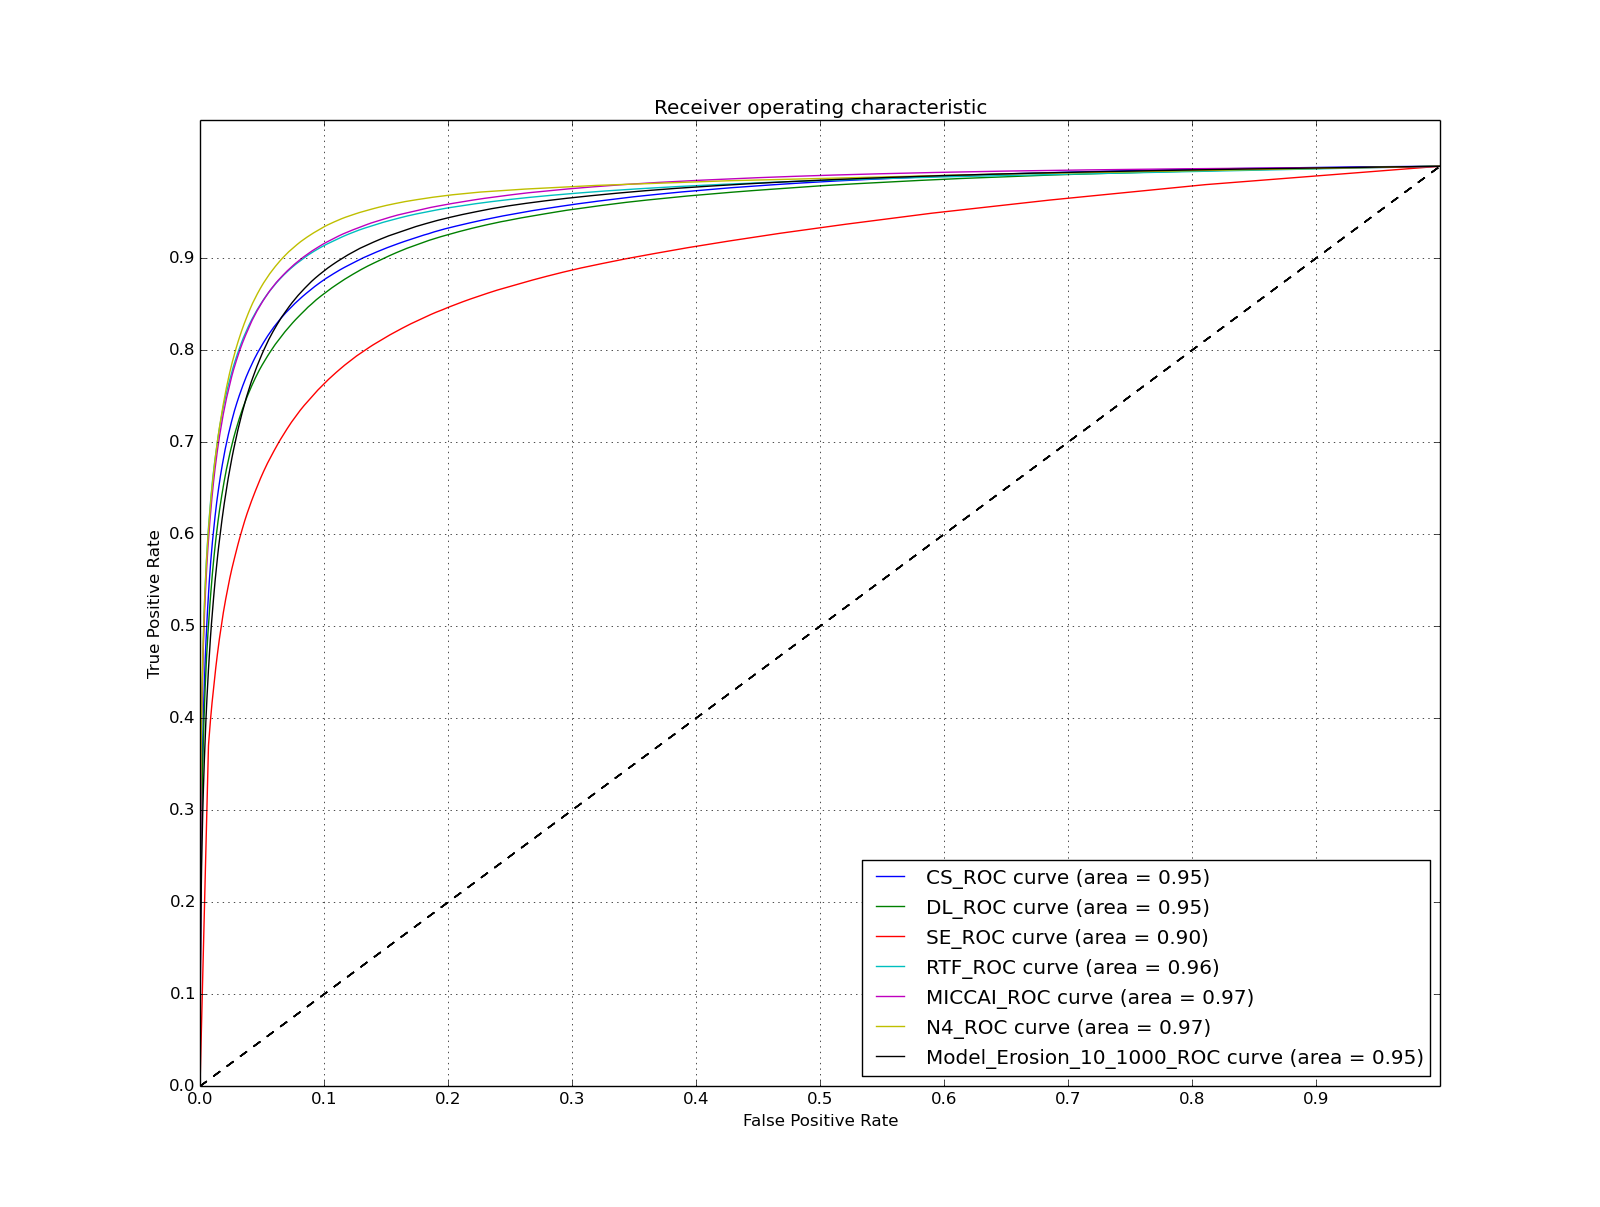
\includegraphics[width=0.8\linewidth]{Images/expt1.png}
\end{figure}
\end{frame}
%-------------------------%
%New frame
%-------------------------%
%------------------------------------------------
\subsection{Expt-1}
\begin{frame}
\frametitle{Comparison with other methods}
\begin{figure}
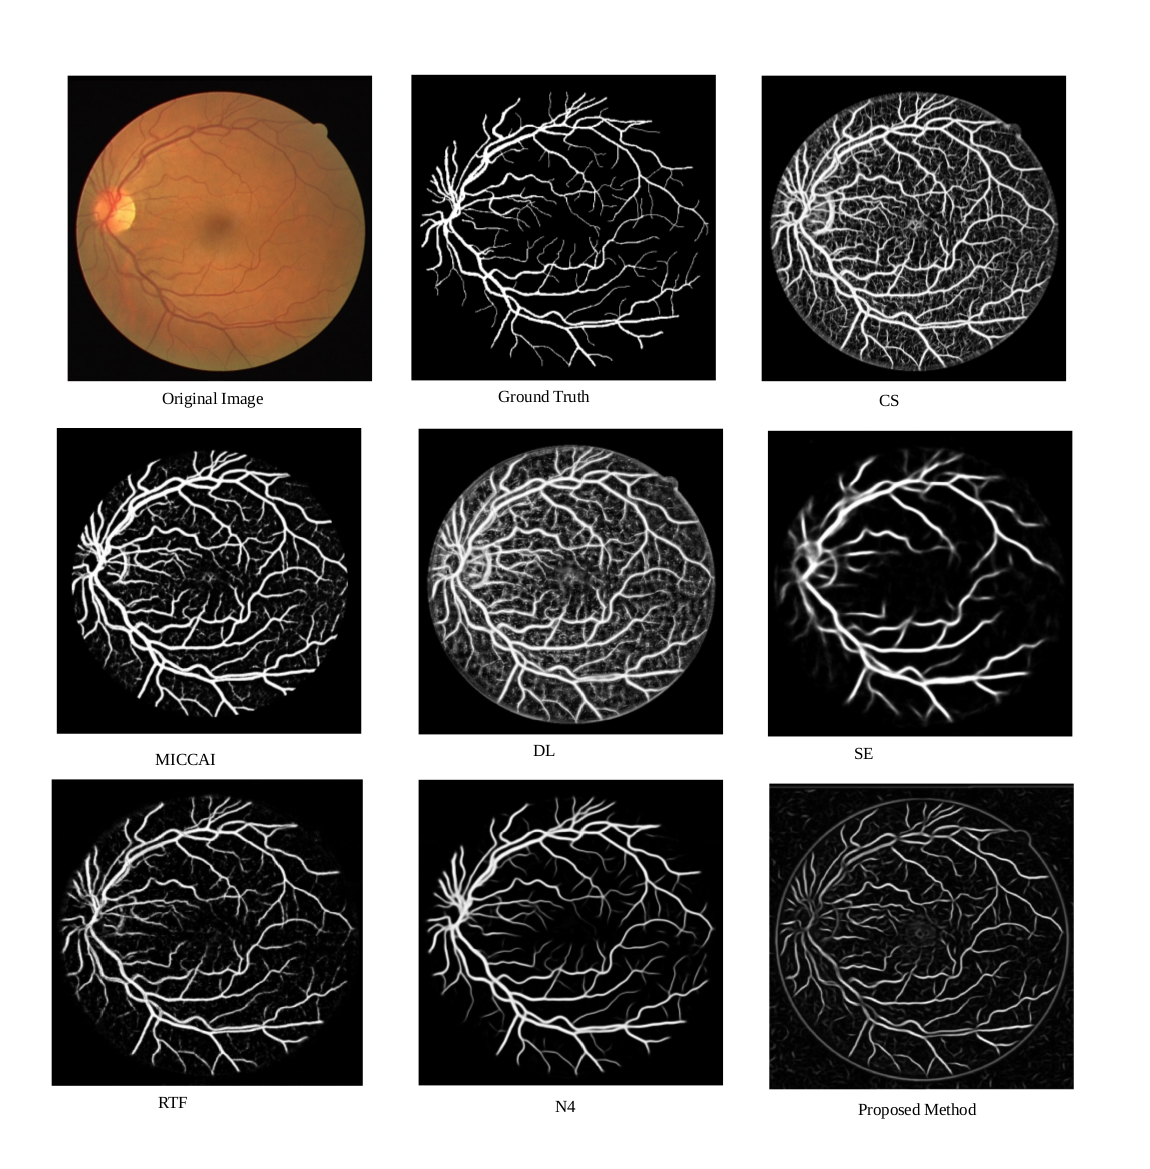
\includegraphics[width=12cm,height=6cm,keepaspectratio]{Images/All_Compare.png}
\end{figure}
\end{frame}
%-------------------------%

\subsection{Method}
\begin{frame}
\frametitle{Comparison with other methods}
\begin{figure}
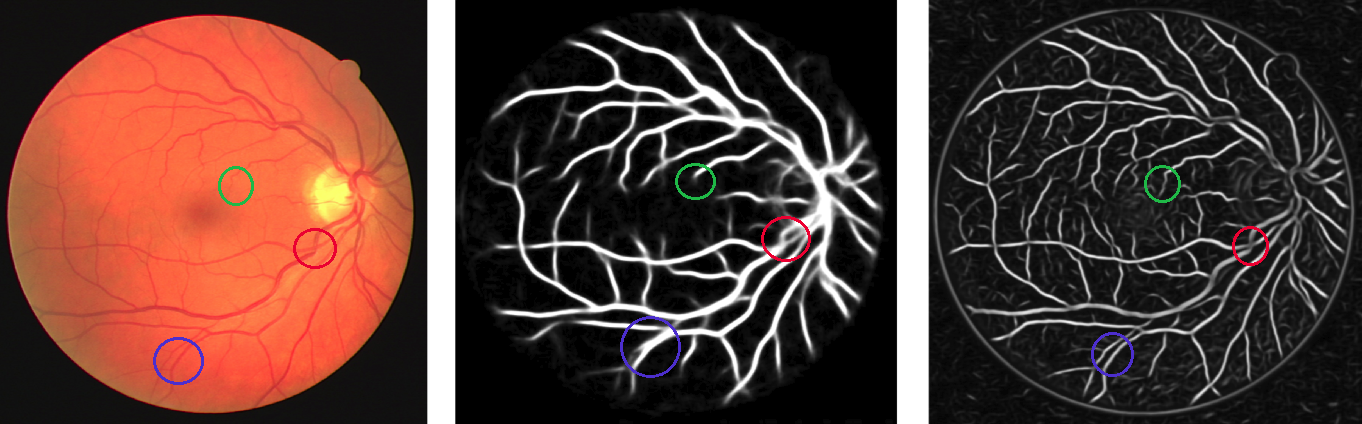
\includegraphics[width=1.0\linewidth]{Images/prob2.png}

\end{figure}

\end{frame}
%-------------------------%
\subsection{Expt-2}
\begin{frame}
\frametitle{Expt2: Cluster Size}
\begin{figure}
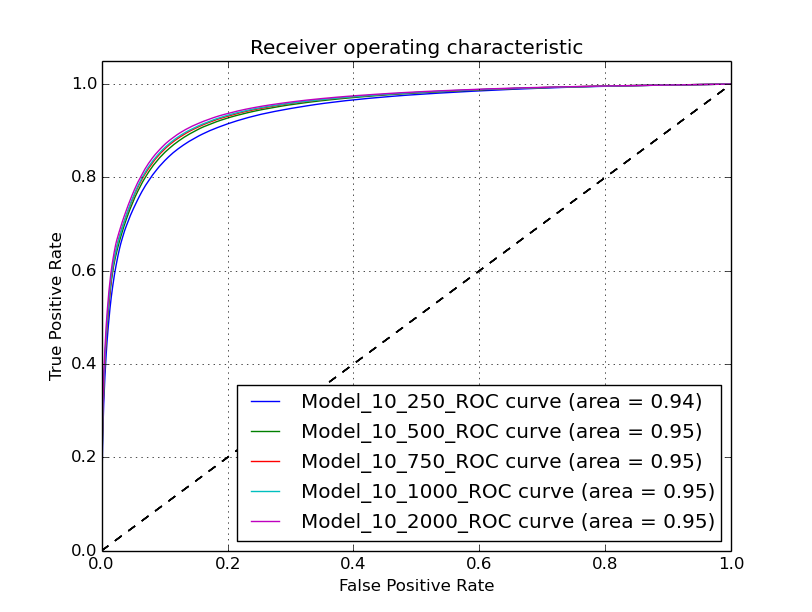
\includegraphics[width=0.8\linewidth]{Images/expt2.png}
\end{figure}
\end{frame}
%-------------------------%
%New frame
%-------------------------%
\subsection{Expt-3}
\begin{frame}
\frametitle{Expt3: Patch Size}
\begin{figure}
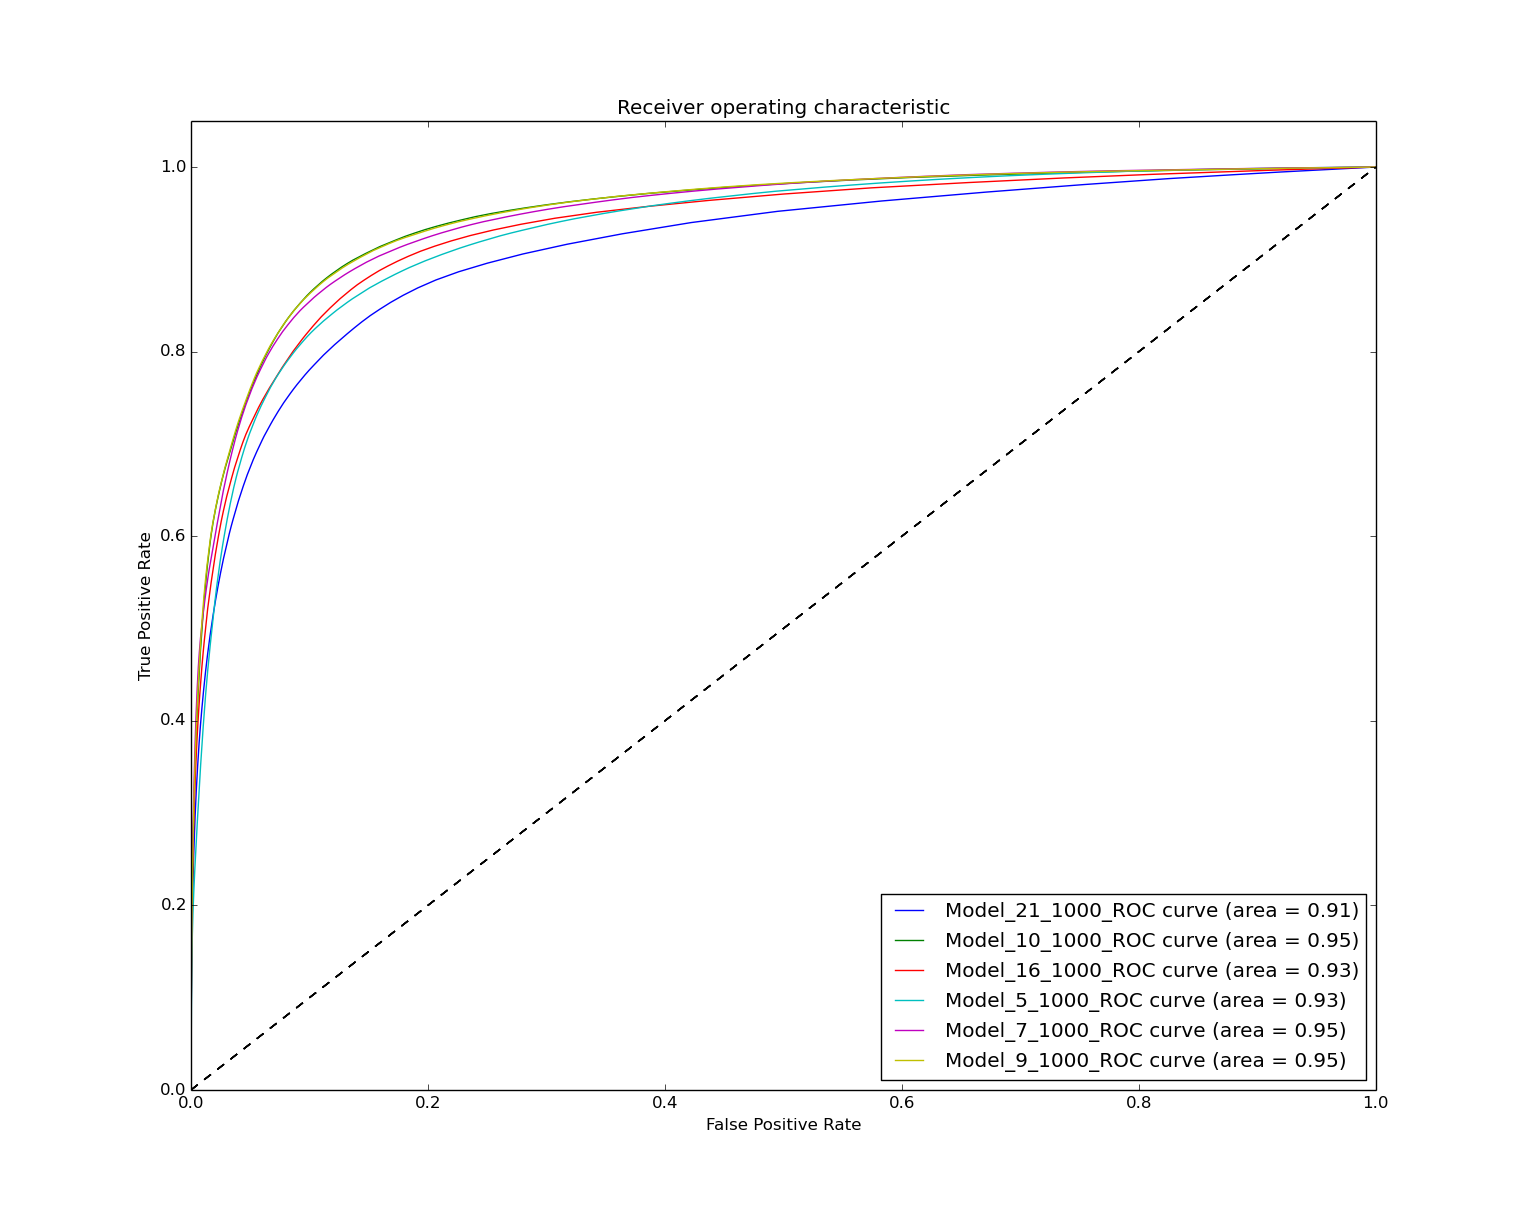
\includegraphics[width=0.8\linewidth]{Images/expt3.png}
\end{figure}
\end{frame}
%-------------------------%
%New frame
%-------------------------%
\subsection{Expt-4}
\begin{frame}
\frametitle{Expt4: Normalization}
\begin{figure}
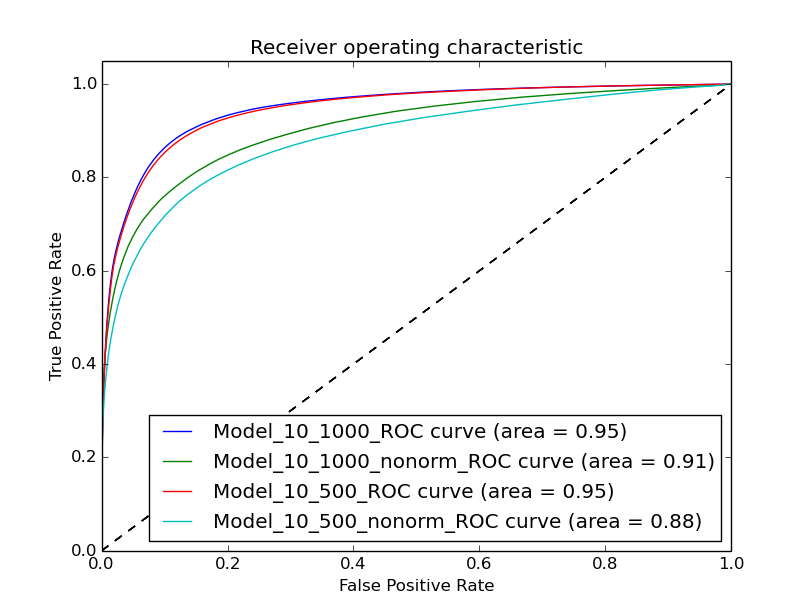
\includegraphics[width=0.8\linewidth]{Images/expt4.png}
\end{figure}
\end{frame}
%-------------------------%
%New frame
%-------------------------%
\subsection{Stare Set}
\begin{frame}
\frametitle{Stare Dataset}
\begin{figure}
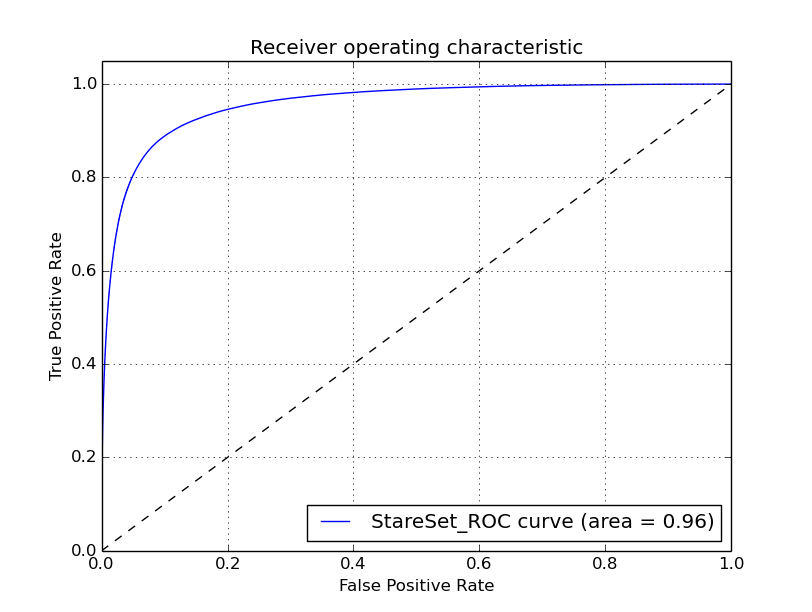
\includegraphics[width=0.8\linewidth]{Images/stare.png}
\end{figure}
\end{frame}
%-------------------------%
%New frame
%-------------------------%

%------------------------------------------------
\section{Questiosns}
%------------------------------------------------
\begin{frame}
\Huge{\centerline{Questions ?}}
\end{frame}

%----------------------------------------------------------------------------------------

\end{document}